\documentclass[landscape,a4paper]{article}
\usepackage{enumerate}
\usepackage{amsmath}
\usepackage{amssymb}
\usepackage{graphicx}
\usepackage{subfigure}
\usepackage{geometry}
\usepackage{caption}
\usepackage{indentfirst}
\usepackage{multicol}

\usepackage{tikz}
\usetikzlibrary{circuits.ee.IEC}
\usetikzlibrary{arrows.meta}
\usetikzlibrary{calc}

\usepackage{minted}
\usepackage{setspace}
\linespread{0.1}

\geometry{left=1cm,right=1cm,top=1cm,bottom=1cm}
\renewcommand{\thesection}{Problem \arabic{section}.}
%\allowdisplaybreaks[4]
\newcommand{\Omegacm}{{\rm\,\Omega\cdot cm}}
\newcommand{\unit}[1]{{\rm\,#1}}

\title{VE311 Homework 8}
\author{Liu Yihao 515370910207}
\date{}

\begin{document}
\pagestyle{empty}

\begin{multicols}{3}
\scriptsize
1.
\begin{center}
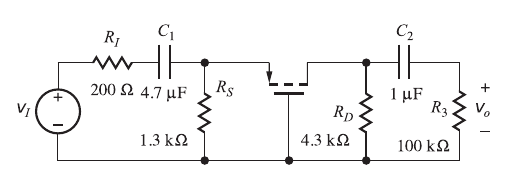
\includegraphics[height=2.5cm]{8.1.png}
\end{center}
$$g_mV=\frac{V_I-V}{R_I+1/C_1s}-\frac{V}{R_S}$$
$$\begin{aligned}V&=\frac{\dfrac{V_I}{R_I+1/C_1s}}{g_m+\dfrac{1}{R_I+1/C_1s}+\dfrac{1}{R_S}}\\&=V_I\cdot\frac{R_S}{R_S+(g_mR_S+1)(R_I+1/C_1s)}\end{aligned}$$
$$V_O=g_mV\cdot\frac{R_D}{R_D+R_3+1/C_2s}\cdot R_3$$
\begin{align*}
\frac{V_O}{V_I}&=g_m\frac{R_S}{R_S+(g_mR_S+1)(R_I+1/C_1s)}\frac{R_D}{R_D+R_3+1/C_2s} R_3\\
&=\frac{g_mR_SR_DR_3C_1sC_2s}{[C_1s(R_S+R_I+g_mR_SR_I)+g_mR_S+1][C_2s(R_D+R_3)+1]}
\end{align*}
$$\omega_{z_1}=\omega_{z_2}=0$$
$$\omega_{p_1}=-\frac{g_mR_s+1}{C_1(R_S+R_I+g_mR_SR_I)}\approx-569.91\unit{rad/s}$$
$$\omega_{p_2}=-\frac{1}{C_2(R_D+R_3)}\approx-9.59\unit{rad/s}$$
$$f_c=\frac{\omega_{p_1}+\omega_{p_2}}{2\pi}\approx92.23\unit{Hz}$$
$$A_{mid}=\frac{g_m(R_D\parallel R_3)}{1+g_m(R_I\parallel R_S)}\cdot\frac{R_S}{R_I+R_S}\approx9.57$$

2.
\begin{center}
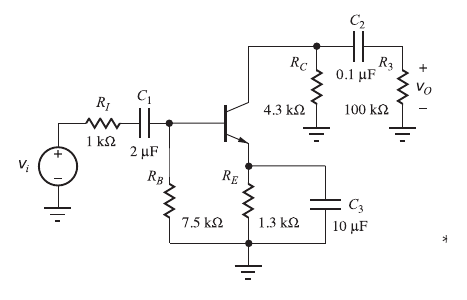
\includegraphics[height=3cm]{8.2.png}
\end{center}
$$g_m=\frac{I_C}{V_T}=\frac{1\unit{mA}}{0.025\unit{V}}=40\unit{mS}$$
$$c_\pi=\frac{g_m}{2\pi f_T}=\frac{40\unit{mS}}{2\pi\cdot500\unit{MHz}}\approx12.73\unit{pF}$$
$$r_\pi=\frac{\beta_0}{g_m}=\frac{100}{40\unit{mS}}=2.5\unit{k\Omega}$$
$$r_{\pi_0}=(R_I\parallel R_B+r_x)\parallel r_\pi=[(1\parallel7.5+0.3)\parallel 2.5]\unit{k\Omega}\approx802\unit{\Omega}$$
$$R_L=R_C\parallel R_3=4.123\unit{k\Omega}$$
$$c_T=c_\pi+c_\mu\left(1+g_mR_L+\frac{R_L}{r_{\pi_0}}\right)=\approx141.03\unit{pF}$$
$$f_{p_1}=\frac{1}{2\pi r_{\pi_0}c_T}=\frac{1}{2\pi\cdot802\unit{\Omega}\cdot141.03\unit{pF}}\approx1.41\unit{MHz}$$
$$f_{p_2}=\frac{g_m}{2\pi c_\pi}=\frac{40\unit{mS}}{2\pi\cdot12.73\unit{pF}}\approx500.09\unit{MHz}$$
$$f_H=f_{p_1}=1.41\unit{MHz}$$
$$A_{mid}=\frac{R_L[R_B\parallel(r_\pi+r_x)]}{R_I+[R_B\parallel(r_\pi+r_x)]}\cdot\frac{-g_mr_\pi}{r_\pi+r_x}\approx-98.79$$
$$GBW=|A_{mid}|f_H=139.29\unit{MHz}$$

3.\\
\begin{minipage}{0.4\linewidth}
\begin{center}
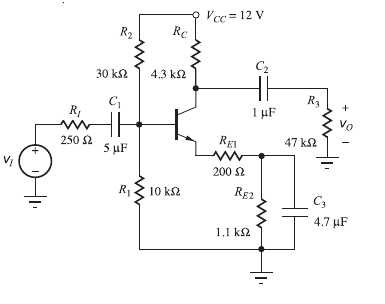
\includegraphics[height=3cm]{8.3.png}
\end{center}
\end{minipage}
\begin{minipage}{0.55\linewidth}
\begin{center}
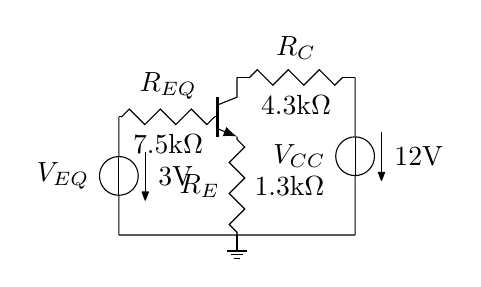
\begin{tikzpicture}[circuit ee IEC,set resistor graphic=var resistor IEC graphic,scale=0.5]
\draw (-0.5,0) to [resistor={ohm=7.5k,info'=$R_{EQ}$}] (-3,0);
\draw (-3,0) to [voltage source={direction info={volt=3},info'=$V_{EQ}$}] (-3,-3);
\draw (3,1) to [voltage source={direction info={volt=12},info'=$V_{CC}$}] (3,-3);
\draw (3,1) to [resistor={ohm=4.3k,info'=$R_C$}] ( 0,1);
\draw (0,-0.5) to [resistor={ohm=1.3k,info'=$R_E$}] (0,-3);
\draw [very thick] (-0.5,0.5) -- (-0.5,-0.5);
\draw (-3,-3) -- (3,-3) (0,1) -- (0,0.5) -- (-0.5, 0.3);
\draw[-{Latex}] (-0.5,-0.3) -- (0,-0.5);
\draw (0,-3.5) node (gnd) [ground,point down] {};
\draw (gnd) -- (0,-3);
\end{tikzpicture}
\end{center}
\end{minipage}
Suppose $V_{BE}=0.7V$,
$$I_C=\frac{V_{EQ}-V_{BE}}{\dfrac{R_{EQ}}{\beta_0}+\dfrac{\beta_0+1}{\beta_0}R_E}\approx1.657\unit{mA}$$
$$I_E=\frac{V_{EQ}-V_{BE}}{\dfrac{R_{EQ}}{\beta_0+1}+R_E}\approx1.673\unit{mA}$$
$$V_{CE}=V_{CC}-I_CR_C-I_ER_E=2.7\unit{V}$$

So the $Q$ point is $(1.657\unit{mA},\ 2.7\unit{V})$.

$$g_m=\frac{I_C}{V_T}=\frac{1.657\unit{mA}}{0.025\unit{V}}=66.28\unit{mS}$$
$$r_\pi=\frac{\beta_0V_T}{I_C}=\frac{100\cdot0.025\unit{V}}{1.657\unit{mA}}\approx1.508\unit{k\Omega}$$
$$r_{\pi_0}=[(R_{EQ}\parallel R_I)+r_x]\parallel[r_\pi+(\beta_0+1)R_E]\approx576\unit{\Omega}$$
$$R_L=R_C\parallel R_3=(4.3\parallel47)\unit{k\Omega}=3.94\unit{k\Omega}$$
$$c_\pi=\frac{g_m}{2\pi f_T}-c_\mu=\frac{66.28\unit{mS}}{2\pi\cdot200\unit{MHz}}-1\unit{pF}\approx51.74\unit{pF}$$
$$c_T=\frac{c_\pi}{1+g_mR_{E}}+c_\mu\left(1+\frac{g_mR_L}{1+g_mR_E+}+\frac{R_L}{r_{\pi_0}}\right)\approx29.79\unit{pF}$$

For $f_H$,
$$f_{p_1}=\frac{1}{2\pi r_{\pi_0}c_T}=\approx9.275\unit{MHz}$$
$$f_{p_2}=\frac{g_m}{2\pi(1+g_mR_E)c_\pi}=\approx14.30\unit{MHz}$$
$$f_{z}=\frac{g_m}{2\pi(1+g_mR_E)c_\mu}=\approx739.95\unit{MHz}$$
$$f_H=\frac{1}{\sqrt{f_{p_1}^{-2}+f_{p_2}^{-2}-2f_{z}^{-2}}}\approx7.78\unit{MHz}$$

For $f_L$,
$$R_{iB}=r_\pi+r_x+(\beta_0+1)R_E=22.06\unit{k\Omega}$$
$$R_{1s}=R_I+R_{EQ}\parallel R_{iB}=\approx5.85\unit{k\Omega}$$
$$R_{2s}=R_3+R_C=(4.3+47)\unit{k\Omega}=51.3\unit{k\Omega}$$
$$R_{3s}=R_{E2}\parallel\left[\frac{r_\pi+r_x+R_I\parallel R_{EQ}}{\beta_0+1}+R_{E1}\right]\approx184\unit{\Omega}$$
$$f_L=\frac{1}{2\pi(R_{1s}C_1)}+\frac{1}{2\pi(R_{2s}C_2)}+\frac{1}{2\pi(R_{3s}C_3}\approx197\unit{Hz}$$

For $A_{mid}$,
$$\begin{aligned}A_{mid}&=\frac{-g_mR_L}{1+g_mR_{E1}}\cdot\frac{R_{EQ}\parallel R_{iB}}{R_I+R_{EQ}\parallel R_{iB}}\\&\cdot\frac{r_\pi+(\beta_0+1)R_{E1}}{r_\pi+r_x+(\beta_0+1)R_{E1}}\approx-17.26\end{aligned}$$

4.
\begin{center}
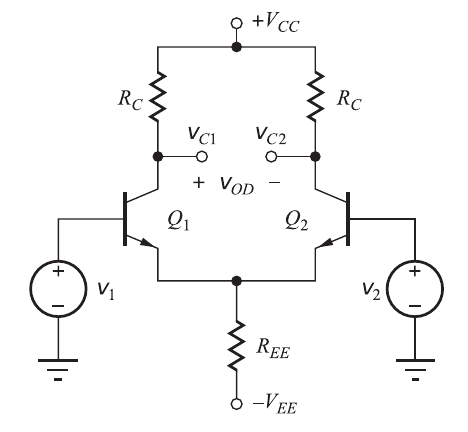
\includegraphics[height=3cm]{6.1.png}
\end{center}
Suppose $V_{BE}=0.7\unit{V}$,
$$I_E=\frac{V_{EE}-V_{BE}}{2R_{EE}}=\frac{18\unit{V}-0.7\unit{V}}{2\cdot47\unit{k\Omega}}\approx0.184\unit{mA}$$
$$I_C=I_E\frac{\beta_F}{\beta_F+1}=0.368\unit{mA}\cdot\frac{100}{101}\approx0.182\unit{mA}$$
$$V_{C}=V_{CC}-I_CR_C=18\unit{V}-0.364\unit{mA}\cdot50\unit{k\Omega}\approx8.9\unit{V}$$
$$V_{CE}=V_{C}+V_{BE}=9.6\unit{V}$$
So the Q point is $(0.184\unit{mA},\ 9.6\unit{V})$.
$$g_m=\frac{I_C}{V_T}=\frac{0.182\unit{mA}}{0.025\unit{V}}=7.28\unit{mS}$$
$$A_{dd}=-g_mR_C=-7.28\unit{mS}\cdot50\unit{k\Omega}=-364$$
$$A_{cc}=-\frac{R_C}{2R_{EE}}=-\frac{50\unit{k\Omega}}{2\cdot47\unit{k\Omega}}\approx-0.53$$
$$CMRR = \frac{A_{dd}}{2A_{cc}} = \frac{-364}{2\cdot -0.53} \approx 343$$
Differential-mode:
$$r_{id}=2r_{\pi}=2\frac{\beta_F}{g_m}=\frac{2\cdot100}{7.28\unit{mS}}\approx27.5\unit{k\Omega}$$
$$r_{od}\approx 2R_C=100\unit{k\Omega}$$
Common-mode:
$$r_{ic}=\frac{r_{\pi}}{2}+(\beta_F+1)R_{EE}=\frac{\beta_F}{2g_m}+(\beta_F+1)R_{EE}\approx4.75\unit{M\Omega}$$
$$r_{oc}\approx R_C=50\unit{k\Omega}$$

5.
\begin{center}
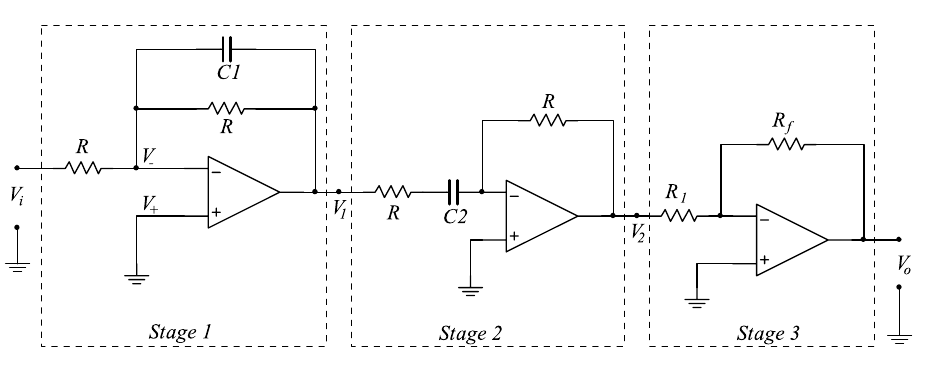
\includegraphics[height=2.5cm]{7.3.png}
\end{center}
Let $s=j\omega$,
$$\frac{V_i}{R}=-\frac{V_1}{R\parallel(1/C_1s)}=-V_1\frac{R+1/C_1s}{R/C_1s}$$
$$\frac{V_1}{V_i}=-\frac{1/C_1s}{R+1/C_1s}=-\frac{1}{RC_1s+1}$$
$$\frac{V_2}{V_1}=-\frac{R}{R+1/C_2s}=-\frac{RC_2s}{RC_2s+1}$$
$$\frac{V_o}{V_2}=-\frac{R_f}{R_1}$$
$$\begin{aligned}\frac{V_o}{V_i}&=\frac{V_1}{V_i}\cdot\frac{V_2}{V_1}\cdot\frac{V_o}{V_2}=-\frac{RR_fC_2s}{R_1(RC_1s+1)(RC_2s+1)}\\&=-\frac{470s}{(47s+1)(0.2s+1)}\end{aligned}$$

The poles are $\omega_{p_1}=-\dfrac{1}{47}\unit{rad/s}$ and $\omega_{p_2}=-5\unit{rad/s}$. The zeros are $\omega_{z_1}=0$.

\end{multicols}

\end{document}

